\documentclass[landscape,a0paper,fontscale=0.292]{baposter}

\usepackage{examples-slim}
\usepackage{amsmath}
\usepackage{amssymb}
\usepackage{booktabs}
\usepackage{colortbl}
\usepackage{url}
\usepackage[normalem]{ulem}
\usepackage{stmaryrd}
\usepackage{natbib}

%=====================================================================
%========================= cross-references ==========================

% Flexible sec/fig/tbl/def cross-refs.
\newcommand{\Secref}[1]{Section~\ref{#1}}
\newcommand{\secref}[1]{section~\ref{#1}}
\newcommand{\dashsecref}[2]{sections~\ref{#1}--\ref{#2}}

\newcommand{\Defref}[1]{Def.~\ref{#1}}
\newcommand{\defref}[1]{def.~\ref{#1}}
\newcommand{\Defrefc}[2]{\Defref{#1}, clause~\ref{#2}}
\newcommand{\defrefc}[2]{\defref{#1}, clause~\ref{#2}}

\newcommand{\Figref}[1]{Figure~\ref{#1}}
\newcommand{\figref}[1]{figure~\ref{#1}}
\newcommand{\dashfigref}[2]{figures~\ref{#1}--\ref{#2}}
\newcommand{\Tabref}[1]{Table~\ref{#1}}
\newcommand{\tabref}[1]{table~\ref{#1}}

% Examples:
\newcommand{\eg}[1]{(\ref{#1})}
\newcommand{\subeg}[2]{(\ref{#1}\ref{#2})}
\newcommand{\dblsubeg}[3]{(\ref{#1}\ref{#2},~\ref{#3})}
\newcommand{\dashsubeg}[3]{(\ref{#1}\ref{#2}--\ref{#3})}

% In-text citations
\newcommand{\posscitet}[1]{\citeauthor{#1}'s~(\citeyear{#1})}
\newcommand{\sposscitet}[1]{\citeauthor{#1}'~(\citeyear{#1})}
\newcommand{\possciteauthor}[1]{\citeauthor{#1}'s}
\newcommand{\spossciteauthor}[1]{\citeauthor{#1}'}
\newcommand{\pgposscitet}[2]{\citeauthor{#1}'s~(\citeyear{#1}:~#2)}
\newcommand{\secposscitet}[2]{\citeauthor{#1}'s~(\citeyear{#1}:~$\S$#2)}
\newcommand{\pgcitealt}[2]{\citealt{#1}:~#2}
\newcommand{\seccitealt}[2]{\citealt{#1}:~$\S$#2}
\newcommand{\pgcitep}[2]{(\citealt{#1}:~#2)}
\newcommand{\seccitep}[2]{(\citealt{#1}:~$\S$#2)}
\newcommand{\pgcitet}[2]{\citeauthor{#1}~(\citeyear{#1}:~#2)}
\newcommand{\seccitet}[2]{\citeauthor{#1}~(\citeyear{#1}:~$\S$#2)}

%=====================================================================
%============================ text styles ============================

\newcommand{\word}[1]{\emph{#1}}
\newcommand{\tech}[1]{\textbf{#1}}
\definecolor{maroon}{HTML}{990000}
\newcommand{\highlight}[1]{{\color{maroon}#1}}

%=====================================================================
%============================== judgments ============================

\newcommand{\bad}{\sqz{${}^\ast$}}
\newcommand{\freebad}{${}^\ast$}
\newcommand{\marked}{\sqz{${}^\#$}}
\newcommand{\freemarked}{${}^\#$}

%=====================================================================
%=============================== model ===============================


\newcommand{\tuple}[1]{\ensuremath{\left< #1 \right>}}
\newcommand{\set}[1]{\ensuremath{\left\{ #1 \right\}}}
\newcommand{\True}{\texttt{T}}
\newcommand{\False}{\texttt{F}}
\newcommand{\Reals}{\mathbb{R}}
\newcommand{\given}{\mid}
\newcommand{\Indicator}{\mathbb{I}}

\newcommand{\sem}[1]{\ensuremath{\llbracket#1\rrbracket}}
\newcommand{\States}{W}
\newcommand{\state}{w}
\newcommand{\Lex}{\mathcal{L}}
\newcommand{\LexStar}{\Lex^{\ast}}
\newcommand{\LexSet}{\mathbf{L}}
\newcommand{\Messages}{M}
\newcommand{\msg}{m}
\newcommand{\Costs}{C}
\newcommand{\Prior}{P}
\newcommand{\LexPrior}{P_{\LexSet}}

\newcommand{\listenerZero}{l_{0}}
\newcommand{\speakerOne}{s_{1}}
\newcommand{\listenerOne}{l_{1}}
\newcommand{\SpeakerK}[1][k]{S_{#1}}
\newcommand{\ListenerK}[1][k]{L_{#1}}

\newcommand{\nullmsg}{\mathbf{0}}

%=====================================================================
%============================ annotations ============================

\let\oldmarginpar\marginpar
\renewcommand{\marginpar}[1]{\oldmarginpar[\color{red}\raggedright\scriptsize #1]{\color{red}\raggedright\scriptsize #1}}

\newcommand{\textnote}[1]{{\color{red}#1}}

%=====================================================================
%============================== colors ===============================

\definecolor{lightgray}{HTML}{CCCCCC} 

\definecolor{highlightcolor}{HTML}{D95F02}
\definecolor{annotationcolor}{HTML}{777777} 
\definecolor{worldinfocolor}{HTML}{E7298A}
\definecolor{lexcolor}{HTML}{D95F02}
\definecolor{costcolor}{HTML}{A6761D}
\definecolor{defcolor}{HTML}{D95F02}
%\definecolor{hurfordcolor}{HTML}{00CC33}
\definecolor{hurfordcolor}{HTML}{1B9E77}
\newcommand{\hurford}[1]{{\relax\color{hurfordcolor}#1}}
\newcommand{\definitional}[1]{\relax{\color{defcolor}#1}}

\newcommand{\graycell}[1]{{\cellcolor[gray]{.8}#1}}

%=====================================================================
%============================== helpers ==============================

\newcommand{\porq}{p\,\word{or}\,q}
\newcommand{\pandq}{p\,\&\,q}

\newcommand{\disjlexicon}[2]{
  \left[
    \begin{array}[c]{l@{ \ \mapsto \ } l}
      \porq    & \set{#1} \\
      \pandq   & \set{#2} \\
      \nullmsg & \set{w_{1}, w_{2}, w_{3}} \\
    \end{array}
  \right]}

\newcommand{\listenerMatrix}[6]{
  \begin{array}[c]{l *{4}{r}}
    \toprule
    #1 & w_{1} & w_{2} & w_{3} \\
    \midrule
    p        & #2 \\
    q        & #3 \\              
    \pandq   & #4 \\
    \porq    & #5 \\
    \nullmsg & #6 \\
    \bottomrule
  \end{array}}

\newcommand{\speakerMatrix}[4]{
  \begin{array}[c]{r *{5}{r}}
    \toprule
    #1 & p & q & \pandq & \porq & \nullmsg \\
    \midrule
    w_{1} & #2 \\
    w_{2} & #3 \\ 
    w_{3} & #4 \\ 
    \bottomrule
  \end{array}}

\newcommand{\ListenerKMatrix}[4]{
  \begin{array}[c]{l *{3}{r}}
  \toprule
    #1 & w_{1} & w_{2} & w_{3} \\
    \midrule
    \LexStar  & #2 \\
    \Lex_{1}  & #3 \\
    \Lex_{2}  & #4 \\
    \bottomrule
  \end{array}}

\newcommand{\SpeakerKMatrix}[4]{
  \begin{array}[c]{l *{3}{r}}
    \toprule
    \Lex_{#1} & \porq & \pandq & \nullmsg \\
    \midrule
    w_{1}  & #2 \\
    w_{2}  & #3 \\
    w_{3}  & #4 \\
    \bottomrule
  \end{array}}

\newcommand{\smalldisjlex}[3]{
  \setlength{\arraycolsep}{1pt}
  \left[
    \begin{array}[c]{l@{ \ \mapsto \ }r@{, \ } l@{ \ \mapsto \ }r@{, \ } l@{ \ \mapsto \ }r}
      A & \set{#1} &
      B & \set{#2} &
      X & \set{#3}
    \end{array}
  \right]}

\newcommand{\smalldisjlexTargetDef}{\smalldisjlex{\definitional{\mathbf{w_{1}}}}{w_{2}}{\definitional{\mathbf{w_{1}}}}}

\newcommand{\smalldisjlexTargetHuford}{\smalldisjlex{\hurford{\mathbf{w_{1}}}}{w_{2}}{\hurford{\mathbf{w_{2}}}}}

\renewcommand{\smallhurfordlex}[3]{
  \setlength{\arraycolsep}{1pt}
  \left[
    \begin{array}[c]{l@{:\, }r@{,\, } l@{:\, }r@{,\, } l@{:\, }r}
      A & \set{#1} &
      B & \set{#2} &
      X & \set{#3}
    \end{array}
  \right]}

\definecolor{highlightcolor}{HTML}{D95F02}
\definecolor{annotationcolor}{HTML}{777777} 
\definecolor{worldinfocolor}{HTML}{E7298A}
\definecolor{lexcolor}{HTML}{D95F02}
\definecolor{costcolor}{HTML}{A6761D}


\definecolor{defcolor}{HTML}{D95F02}
\definecolor{hurfordcolor}{HTML}{00CC33}
\newcommand{\hurford}[1]{{\relax\color{hurfordcolor}#1}}
\newcommand{\definitional}[1]{\relax{\color{defcolor}#1}}

\renewcommand{\highlight}[1]{{\color{highlightcolor}#1}}

\newcommand{\lisZeroDef}{\listenerZero(\state \given \msg, \Lex) \propto \frac{\Indicator(\state \in \Lex(\msg))}{|\Lex(\msg)|}\Prior(\state)}
\newcommand{\spkOneDef}{\speakerOne(\msg \given \state, \Lex) \propto \exp\left(\log\left(\alpha\,\listenerZero(\state \given \msg, \Lex) \right)- \gamma\,\Costs(\msg)\right)}
\newcommand{\lisOneDef}{\listenerOne(\state \given \msg, \Lex) \propto \speakerOne(\msg \given \state, \Lex)\Prior(\state)}
\newcommand{\LisOneDef}{%
  \setlength{\arraycolsep}{1pt}%
  %\begin{array}[t]{r c l}
    \ListenerK[1](\state, \Lex \given \msg) = {\color{worldinfocolor}\ListenerK(\state \given \msg, \Lex)} {\color{lexcolor}\ListenerK(\Lex \given \msg)}% \\
    %\ListenerK(\Lex \given \msg) &\propto&  \Prior(\Lex) \sum_{\state\in\States} \SpeakerK(\msg \given \state, \Lex)\Prior(\state)
  %\end{array}
  }
\newcommand{\SpkTwoDef}{\SpeakerK[2](\msg \given \state, \Lex) \propto 
  \exp\left(
    \log
    \left({\color{worldinfocolor}\alpha\,\ListenerK[k-1](\state \given \msg, \Lex)}\right)
    -
    {\color{lexcolor}\beta \log\left(\ListenerK[k-1](\Lex\given\msg)\right)}
    -
    {\color{costcolor}\gamma\,\Costs(\msg)}
  \right)}

\newcommand{\lismat}[4]{
  \setlength{\arraycolsep}{1pt}
  \begin{array}[c]{l *{3}{r}}
    \toprule
    #1 & w_{1} & w_{2} & w_{1}{\vee}w_{2} \\
    \midrule
    A & #2\\
    X & #3 \\
    A\, \word{or}\, X & #4 \\
    \bottomrule
  \end{array}}

\newcommand{\spkmat}[4]{
  \setlength{\arraycolsep}{1pt}
  \begin{array}[c]{l *{3}{r}}
    \toprule
    #1 & A & X & A\, \word{or}\, X\\
    \midrule
    w_{1} & #2\\
    w_{2} & #3 \\
    w_{1}{\vee}w_{2} & #4 \\
    \bottomrule
  \end{array}}
 
\newcounter{excounter}
\setcounter{excounter}{0}
\newcommand{\exitem}[1]{\refstepcounter{excounter}(\theexcounter)\label{#1}}

\definecolor{lightgray}{HTML}{CCCCCC} 
\renewcommand{\graycell}[1]{\colorbox{lightgray}{#1}}

\newcommand{\whitecell}[1]{\colorbox{white}{#1}}

\renewcommand{\state}{w}


%%%%%%%%%%%%%%%%%%%%%%%%%%%%%%%%%%%%%%%%%%%%%%%%%%%%%%%%%%%%%%%%%%%%%%
%%%%%%%%%%%%%%%%%%%%%%%%%%%%%%%%%%%%%%%%%%%%%%%%%%%%%%%%%%%%%%%%%%%%%%

\begin{document}
\begin{poster}{
    % Show grid to help with alignment
    grid=false,
    % Column spacing
    colspacing=0.7em,
    % Color style
    headerColorOne=cyan!20!white!90!black,
    borderColor=cyan!30!white!90!black,
    % Format of textbox
    textborder=faded,
    % Format of text header
    eyecatcher=false,
    headerborder=open,
    headershape=roundedright,
    headershade=plain,
    background=none,
    bgColorOne=cyan!10!white,
    headerheight=0.09\textheight
}
{} % Eye Catcher
{Negotiating lexical uncertainty and expertise with disjunction\vspace{0.25em}}
{Roger Levy and Christopher Potts}
{
\includegraphics[height=0.08\textheight]{stanford}
 \hspace{-10pt}
 
\includegraphics[height=0.08\textheight]{ucsd}
}

%%%%%%%%%%%%%%%%%%%%%%%%%%%%%%%%%%%%%%%%%%%%%%%%%%%%%%%%%%%%%%%%%%%%%%
\headerbox{Communicating in language about language}{name=intro,column=0,row=0,span=2}{

  \begin{itemize}\setlength{\itemsep}{0pt}
  \item Languages are neither fixed across time nor identically
    reproduced in all speakers, but rather continually renegotiated
    during interactions \cite{Clark97}.

  \item People accommodate to each other's usage patterns
    \cite{Giles:Coupland:Coupland:1991}, form temporarily lexical
    pacts \cite{Clark:Wilkes-Gibbs:1986,Brennan:Clark:1996}, and
    instruct each other about their linguistic views
    \cite{Hearst92,SnowEtAl05}.

  \item Some of this communication in language about language is
    direct, as with explicit definitions, but much of it arrives via
    secondary pragmatic inferences.

  \item Disjunction supports what appear to be opposing inferences
    about language:

    \vspace{-5pt}

    \begin{itemize}\setlength{\itemsep}{0pt}
    \item \textbf{Hurfordian pressure \cite{Hurford:1974}:} \word{X or
        Y} conveys that \word{X} and \word{Y} are disjoint
    \item \textbf{Definitional inference \cite{Horn89}:} \word{X or Y}
      conveys that \word{X} and \word{Y} are synonymous
    \end{itemize}

    \vspace{-5pt}
    
  \item This pattern is cross-linguistically robust, so we seek a
    single pragmatic model that can derive both of these meanings from
    the semantics of disjunction given different contextual
    assumptions.
  \end{itemize}

}

%%%%%%%%%%%%%%%%%%%%%%%%%%%%%%%%%%%%%%%%%%%%%%%%%%%%%%%%%%%%%%%%%%%%%%
\headerbox{Hurfordian perceptions and intentions}{name=hurford,column=0,row=2,span=2,below=intro}{

  \textbf{Generalization}: \word{X or Y} conveys that the speaker is
  using a lexicon in which \word{X} and \word{Y} are disjoint, or it
  addresses a speaker concern that the listener is using such a
  lexicon.

  \vspace{4pt}

  \begin{minipage}[c]{0.48\linewidth}
    \renewcommand{\arraystretch}{1.2}
    \begin{tabular}[c]{r@{ \ } p{0.85\textwidth}}
    \exitem{1} & the nuptials will take place in either \hurford{France or Paris} \\
    \exitem{2} & the \hurford{canoe or boat} will be held by the stream's current \\
    \exitem{3} & In 1940, 37\% of us had gone to a \hurford{church or synagogue} in the last week.
    \end{tabular}

    \begin{center}      
      \begin{tabular}[c]{@{} p{3cm} @{}} 
        No clear evidence for ordering restrictions or preferences
        deriving from the entailment relation:
      \end{tabular}
      \renewcommand{\arraystretch}{1}
      \begin{tabular}[c]{l r}
        \toprule
        \multicolumn{2}{c}{\textbf{Our corpus}} \\
        Disjunct order & Exs. \\
        \midrule
        {}[general] or [specific] & 75 \\
        {}[specific] or [general] & 86 \\
        \bottomrule
      \end{tabular}      
    \end{center}       
  \end{minipage}
  \hfill 
  \begin{minipage}[c]{0.45\linewidth}  
    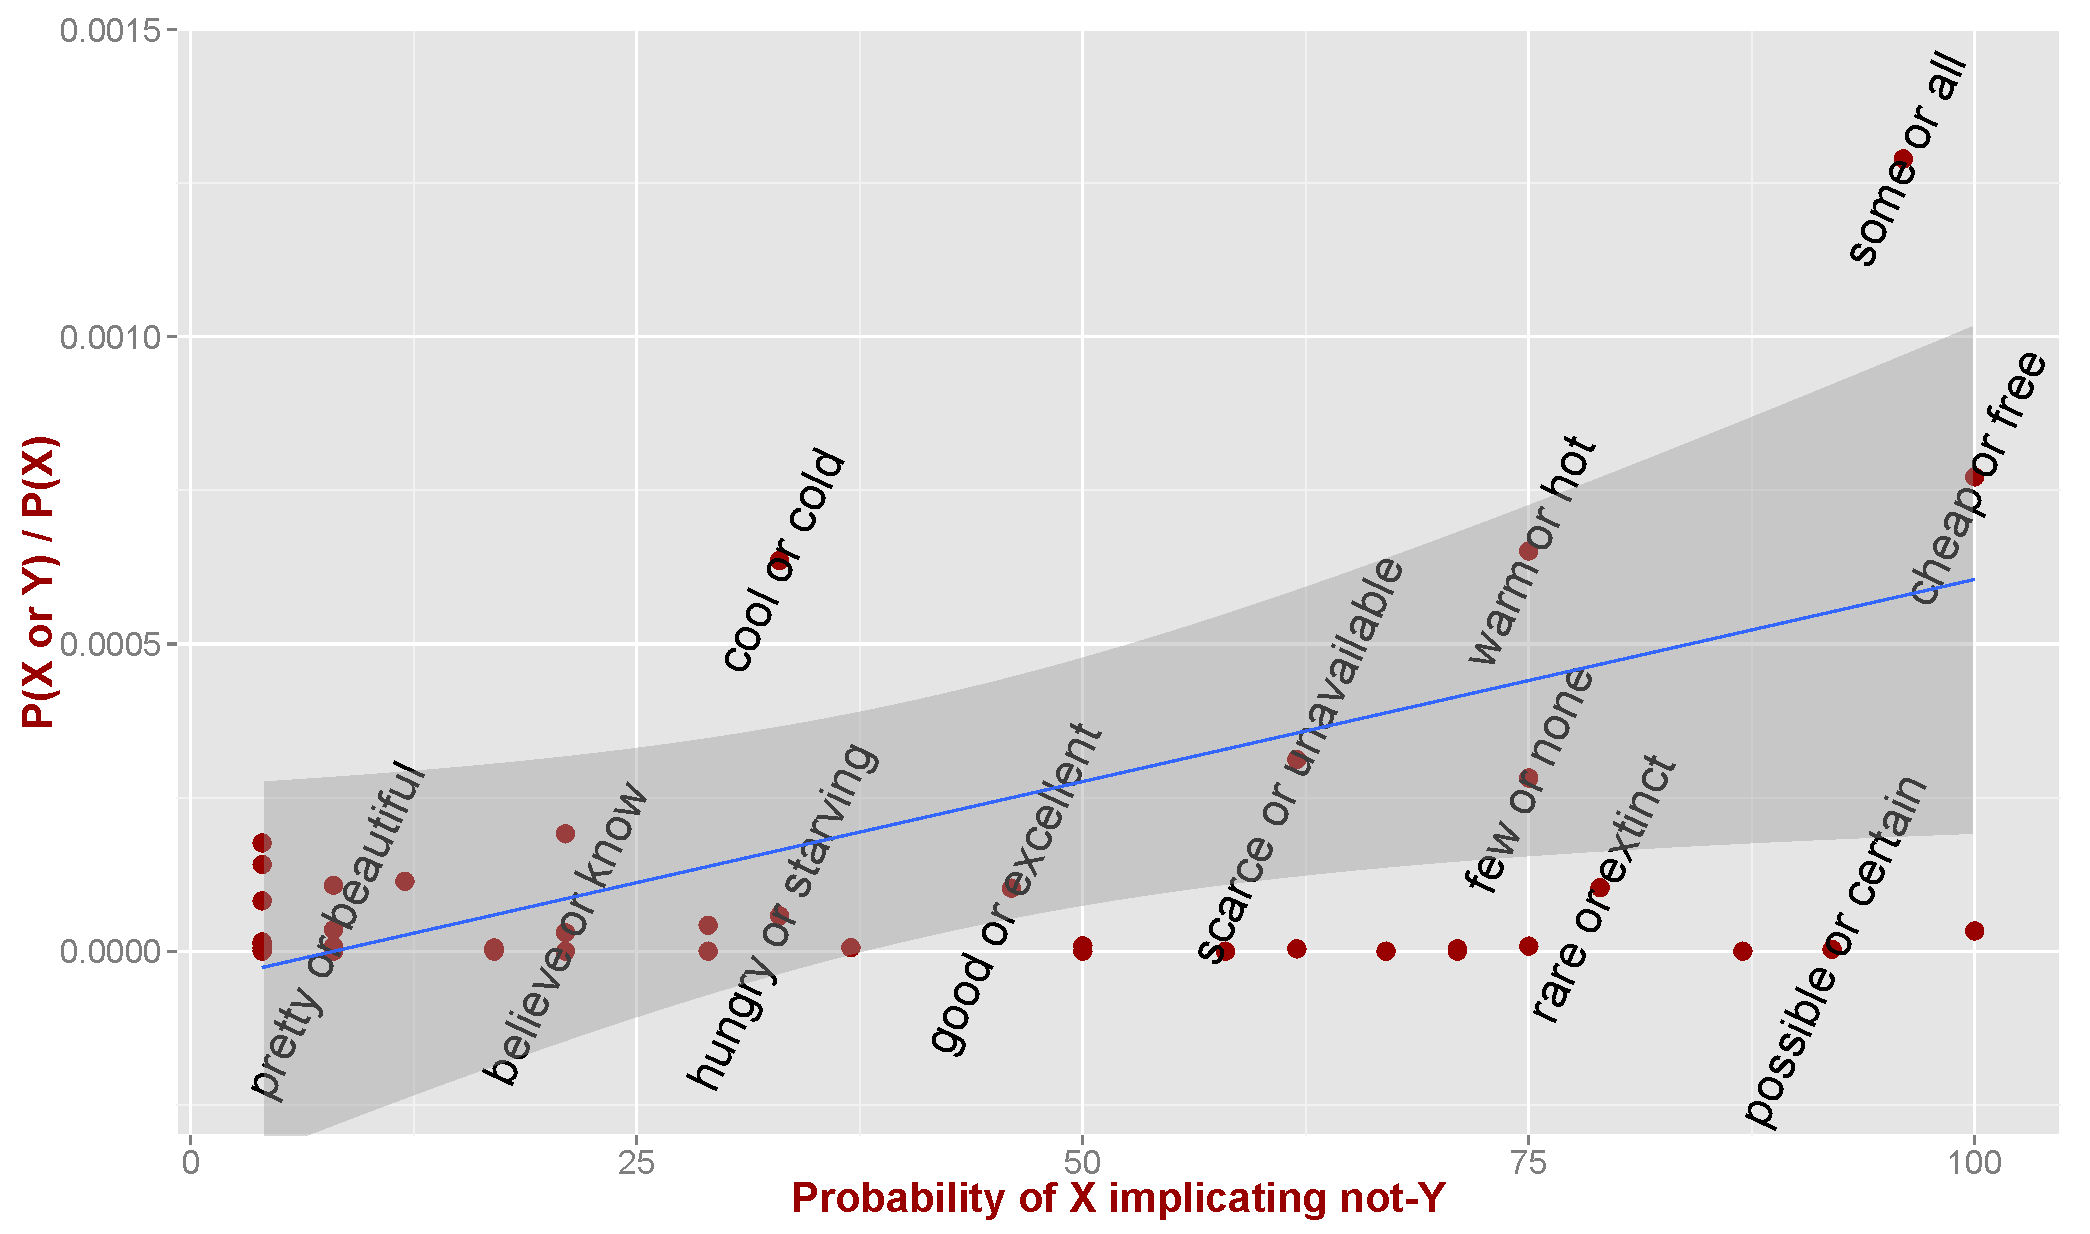
\includegraphics[width=1\textwidth]{chemla-poster.pdf} \\
    The frequency of \word{X or Y} usage correlates with the
    prevalence of \word{X} implicating \word{not Y}
    \cite{Chemla-HurfordCounts}.
  \end{minipage}

}

%%%%%%%%%%%%%%%%%%%%%%%%%%%%%%%%%%%%%%%%%%%%%%%%%%%%%%%%%%%%%%%%%%%%%%
\headerbox{Disjunctive definition and identification}{name=def,column=0,row=2,span=2,below=hurford}{

  \textbf{Generalization}: \word{X or Y} can convey $\sem{X}\approx\sem{Y}$
  when the speaker is mutually, publicly known to be an expert or
  would like to establish expertise.

  \vspace{6pt}

  \begin{minipage}[c]{0.48\linewidth}
    \renewcommand{\arraystretch}{1.2}
    \begin{tabular}[t]{r@{ \ } p{0.85\textwidth}}
    \exitem{4} & She's a \definitional{wine lover or \emph{oenophile}}. \\
    \exitem{5} & Title: \definitional{A Geological History of Manhattan or New York Island} \\
    \exitem{6} & Welcome to \definitional{New Haven or ``the Elm City''}.  \\
    \exitem{7} & It's a \definitional{woodchuck, or land beaver}.
    \end{tabular}    
  \end{minipage}
  \hfill 
  \begin{minipage}[c]{0.48\linewidth}
    \begin{itemize}\setlength{\itemsep}{0pt}
    \item Motivation: speaker is a known `instructor'; listener is a known non-expert.
    \item Motivation: speaker wishes to display expertise to another expert.
    \item Motivation: speaker sees value in (temporarily or permanently) defining a term.
    \end{itemize}    
  \end{minipage}
  
  \vspace{6pt}

  Attested in Chinese, German, Hebrew, Ilokano, Japanese, Russian, and
  Tagalog. Seems to survive even where the language has a dedicated
  definitional disjunction morpheme (e.g., Finnish, Italian).  

}

%%%%%%%%%%%%%%%%%%%%%%%%%%%%%%%%%%%%%%%%%%%%%%%%%%%%%%%%%%%%%%%%%%%%%%
\headerbox{Further information}{name=info,column=0,row=3,span=2,below=def}{  
  
  Paper, references, model code, corpus data: \url{http://github.com/cgpotts/pypragmods/}

}


%%%%%%%%%%%%%%%%%%%%%%%%%%%%%%%%%%%%%%%%%%%%%%%%%%%%%%%%%%%%%%%%%%%%%%
%%%%%%%%%%%%%%%%%%%%%%%%%%%%%%%%%%%%%%%%%%%%%%%%%%%%%%%%%%%%%%%%%%%%%%
\headerbox{Modeling communication with anxious experts}{name=model,column=2,row=0,span=2}{

  \newcommand{\labelednode}[2]{\put(#1){\makebox(0,0)[l]{#2}}}
  \newcommand{\annotation}[2]{\labelednode{#1}{{\footnotesize #2}}}
  \newcommand{\picarrow}[3][1.8]{\put(#2){\vector(#3){#1}}}

  \setlength{\unitlength}{1cm}
  \begin{picture}(16,7.25)

    \labelednode{2,7.2}{$\ldots$}
    \picarrow{2, 7.1}{-2,-1}
    
    \annotation{4,6.45}{{\color{worldinfocolor}world information} $-$ {\color{lexcolor}lexical preferences} $-$ {\color{costcolor}costs}}

    \labelednode{0,5.95}{$\SpkTwoDef$}
    \picarrow{0.2, 5.75}{2,-1}
        
    \annotation{4,4.2}{{\color{worldinfocolor}world information} $*$ {\color{lexcolor}lexical discrimination}}

    \labelednode{2,4.7}{$\LisOneDef$}
    \picarrow[1.3]{2.2, 4.5}{0,-1}
   
    \labelednode{2,2.95}{$\lisOneDef$}
    \picarrow{2, 2.75}{-2,-1}
    
    \labelednode{0,1.7}{$\spkOneDef$}
    \picarrow{0.2, 1.5}{2,-1}
    
    \labelednode{2,0.45}{$\lisZeroDef$}

    {\color{annotationcolor}      
      \labelednode{11.75,4.7}{\parbox{4cm}{suffices for manner implicature and embedded scalar implicature \cite{Smith:Goodman:Frank:2013,bergen-levy-goodman:2014}}}
      \picarrow[1]{11.55, 4.7}{-1,0}
      \labelednode{11.75,2.95}{\parbox{3.8cm}{suffices for unembedded scalar implicature \cite{Frank:Goodman:2012}}}
      \picarrow[1]{11.55, 2.95}{-1,0}
      \labelednode{11.75,1.7}{\parbox{3.8cm}{suffices for many kinds of ambiguity avoidance}}
      \picarrow[1]{11.55, 1.7}{-1,0}
      \labelednode{11.75,0.45}{\parbox{3.8cm}{literal listener, a simple semantic agent}}
      \picarrow[1]{11.55, 0.45}{-1,0}      
    }
  \end{picture}

}

%%%%%%%%%%%%%%%%%%%%%%%%%%%%%%%%%%%%%%%%%%%%%%%%%%%%%%%%%%%%%%%%%%%%%%
\headerbox{Definitional contexts}{name=defmodel,column=2,row=2,span=1,below=model}{  

  Require low disjunction costs and high $\beta$: the speaker is
  invested in communicating about the lexicon and can tolerate the
  cost of a disjunction that is synonymous with one of its disjuncts.

  \vspace{8pt}
     
  \tiny
  \setlength{\tabcolsep}{2pt}
  \setlength{\arraycolsep}{2pt}
  \begin{tabular}[c]{@{}  r@{ }c c c  @{}} 
    \multicolumn{4}{c}{
      \normalsize
      $\begin{array}[c]{l@{ }l r r r}
         \toprule
         & \ListenerK[2] \text{ hears } \word{A\,or\,X}       & w_{1} & w_{2} & w_{1}{\vee}w_{2} \\
         \midrule
         \LexStar & \smallhurfordlex{w_{1}}{w_{2}}{w_{1}, w_{2}}                              & \whitecell{0}   & 0 & .08 \\[1ex]
         \Lex_{1} & \smallhurfordlex{w_{1}}{w_{2}}{w_{2}}                                     & \whitecell{.07} & 0 & .08 \\[1ex]
         \Lex_{2} & \smallhurfordlex{\definitional{\mathbf{w_{1}}}}{w_{2}}{\definitional{\mathbf{w_{1}}}} &  \graycell{.77} & 0 & .06 \\
         \bottomrule
       \end{array}$} \\
    \multicolumn{4}{r}{\normalsize\phantom{a}~\hfill
   $\alpha = 5$; 
   $\beta = 7$; 
   $\Costs(\word{or}) = .01$} 
    \\
    & \multicolumn{3}{c}{$\downarrow$}
    \\    
    & \multicolumn{3}{c}{
    $\begin{array}[c]{r l}
       \toprule
       \multicolumn{2}{c}{\SpeakerK[2] \text{ observes } \langle \Lex_{2},w_{1}\rangle} \\
       \midrule
       A & \phantom{.0}0 \\
       X & \phantom{.0}0 \\
       A\, \word{or}\, X & .05 \\
       \bottomrule
     \end{array}$}
    \\
    & \multicolumn{3}{c}{$\downarrow$}
    \\
    & \multicolumn{3}{c}{
      $\begin{array}[c]{l@{ }l r r r}
         \toprule
         & \ListenerK[1] \text{ hears } \word{A\,or\,X}      & w_{1} & w_{2} & w_{1}{\vee}w_{2} \\
         \midrule
         \LexStar & \smallhurfordlex{w_{1}}{w_{2}}{w_{1}, w_{2}} & 0 & 0 & .23 \\[1ex]
         \Lex_{1} & \smallhurfordlex{w_{1}}{w_{2}}{w_{2}}        & 0 & 0 & .38 \\[1ex]
         \Lex_{2} & \smallhurfordlex{w_{1}}{w_{2}}{w_{1}}        & .38 & 0 & 0\\
         \bottomrule
       \end{array}$}
    \\
    & \multicolumn{3}{c}{$\swarrow \hspace{45pt} \downarrow\hspace{45pt} \searrow$}
    \\
    $\listenerOne$ & $\lismat{\LexStar}{1 & 0 & 0}{02 & 02 & .96}{.02 & .02 & .96}$ &  $\lismat{\Lex_{1}}{1 & 0 & 0}{0 & 1 & 0}{.01 & 0 & .98}$ & $\lismat{\Lex_{2}}{1 & 0 & 0}{1 & 0 & 0}{1 & 0 & 0}$
    \\
    & $\downarrow$ & $\downarrow$ & $\downarrow$
    \\
    $\speakerOne$ & $\spkmat{\LexStar}{.98 & 0 & 0}{0 & 0 & .2}{0 & 0 & .2}$ & $\spkmat{\Lex_{1}}{.99 & 0 & 0}{0 & .33 & 0}{0 & 0 & .33}$ & $\spkmat{\Lex_{2}}{.33 & 0 & 0}{.33 & 0 & 0}{.33 & 0 & 0}$
    \\
    & $\downarrow$ & $\downarrow$ & $\downarrow$
    \\
    $\listenerZero$ & $\lismat{\LexStar}{1 & 0 & 0}{.33 & .33 & .33}{.33 & .33 & .33}$ & $\lismat{\Lex_{1}}{1 & 0 & 0}{0 & 1 & 0}{.33 & .33 & .33}$ & $\lismat{\Lex_{2}}{1 & 0 & 0}{1 & 0 & 0}{1 & 0 & 0}$
  \end{tabular}

}

%%%%%%%%%%%%%%%%%%%%%%%%%%%%%%%%%%%%%%%%%%%%%%%%%%%%%%%%%%%%%%%%%%%%%%
\headerbox{Hurfordian contexts}{name=hurfordmodel,column=3,row=1,span=1,below=model}{
  
  With high disjunction costs, exclusivization maximizes the
  justification for the long form; the Hurfordian instinct is a
  rational response to a disjunction that is unduly prolix for many
  lexica.
  
  \vspace{8pt}
    
  \setlength{\arraycolsep}{2pt}
  $\begin{array}[c]{l@{ }l r r r}
     \toprule
     & \ListenerK[2] \text{ hears } \word{A\, or\, X}       & w_{1} & w_{2} & w_{1}{\vee}w_{2} \\
     \midrule
     \LexStar & \smallhurfordlex{w_{1}}{w_{2}}{w_{1}, w_{2}} & .03 & 0 & \whitecell{.14} \\[1ex]
     \Lex_{1} & \smallhurfordlex{\hurford{\mathbf{w_{1}}}}{w_{2}}{\hurford{\mathbf{w_{2}}}} & .04 & 0 & \graycell{.45} \\[1ex]
     \Lex_{2} & \smallhurfordlex{w_{1}}{w_{2}}{w_{1}} & .02 & 0 & \whitecell{.32} \\
     \bottomrule
   \end{array}$  
   \phantom{a}~\hfill
   $\alpha = 2$; 
   $\beta = 1$; 
   $\Costs(\word{or}) = 1$

   \vspace{-6pt}

}

%%%%%%%%%%%%%%%%%%%%%%%%%%%%%%%%%%%%%%%%%%%%%%%%%%%%%%%%%%%%%%%%%%%%%%
\headerbox{Characterization}{name=char,column=3,row=4,span=1,below=hurfordmodel}{  
  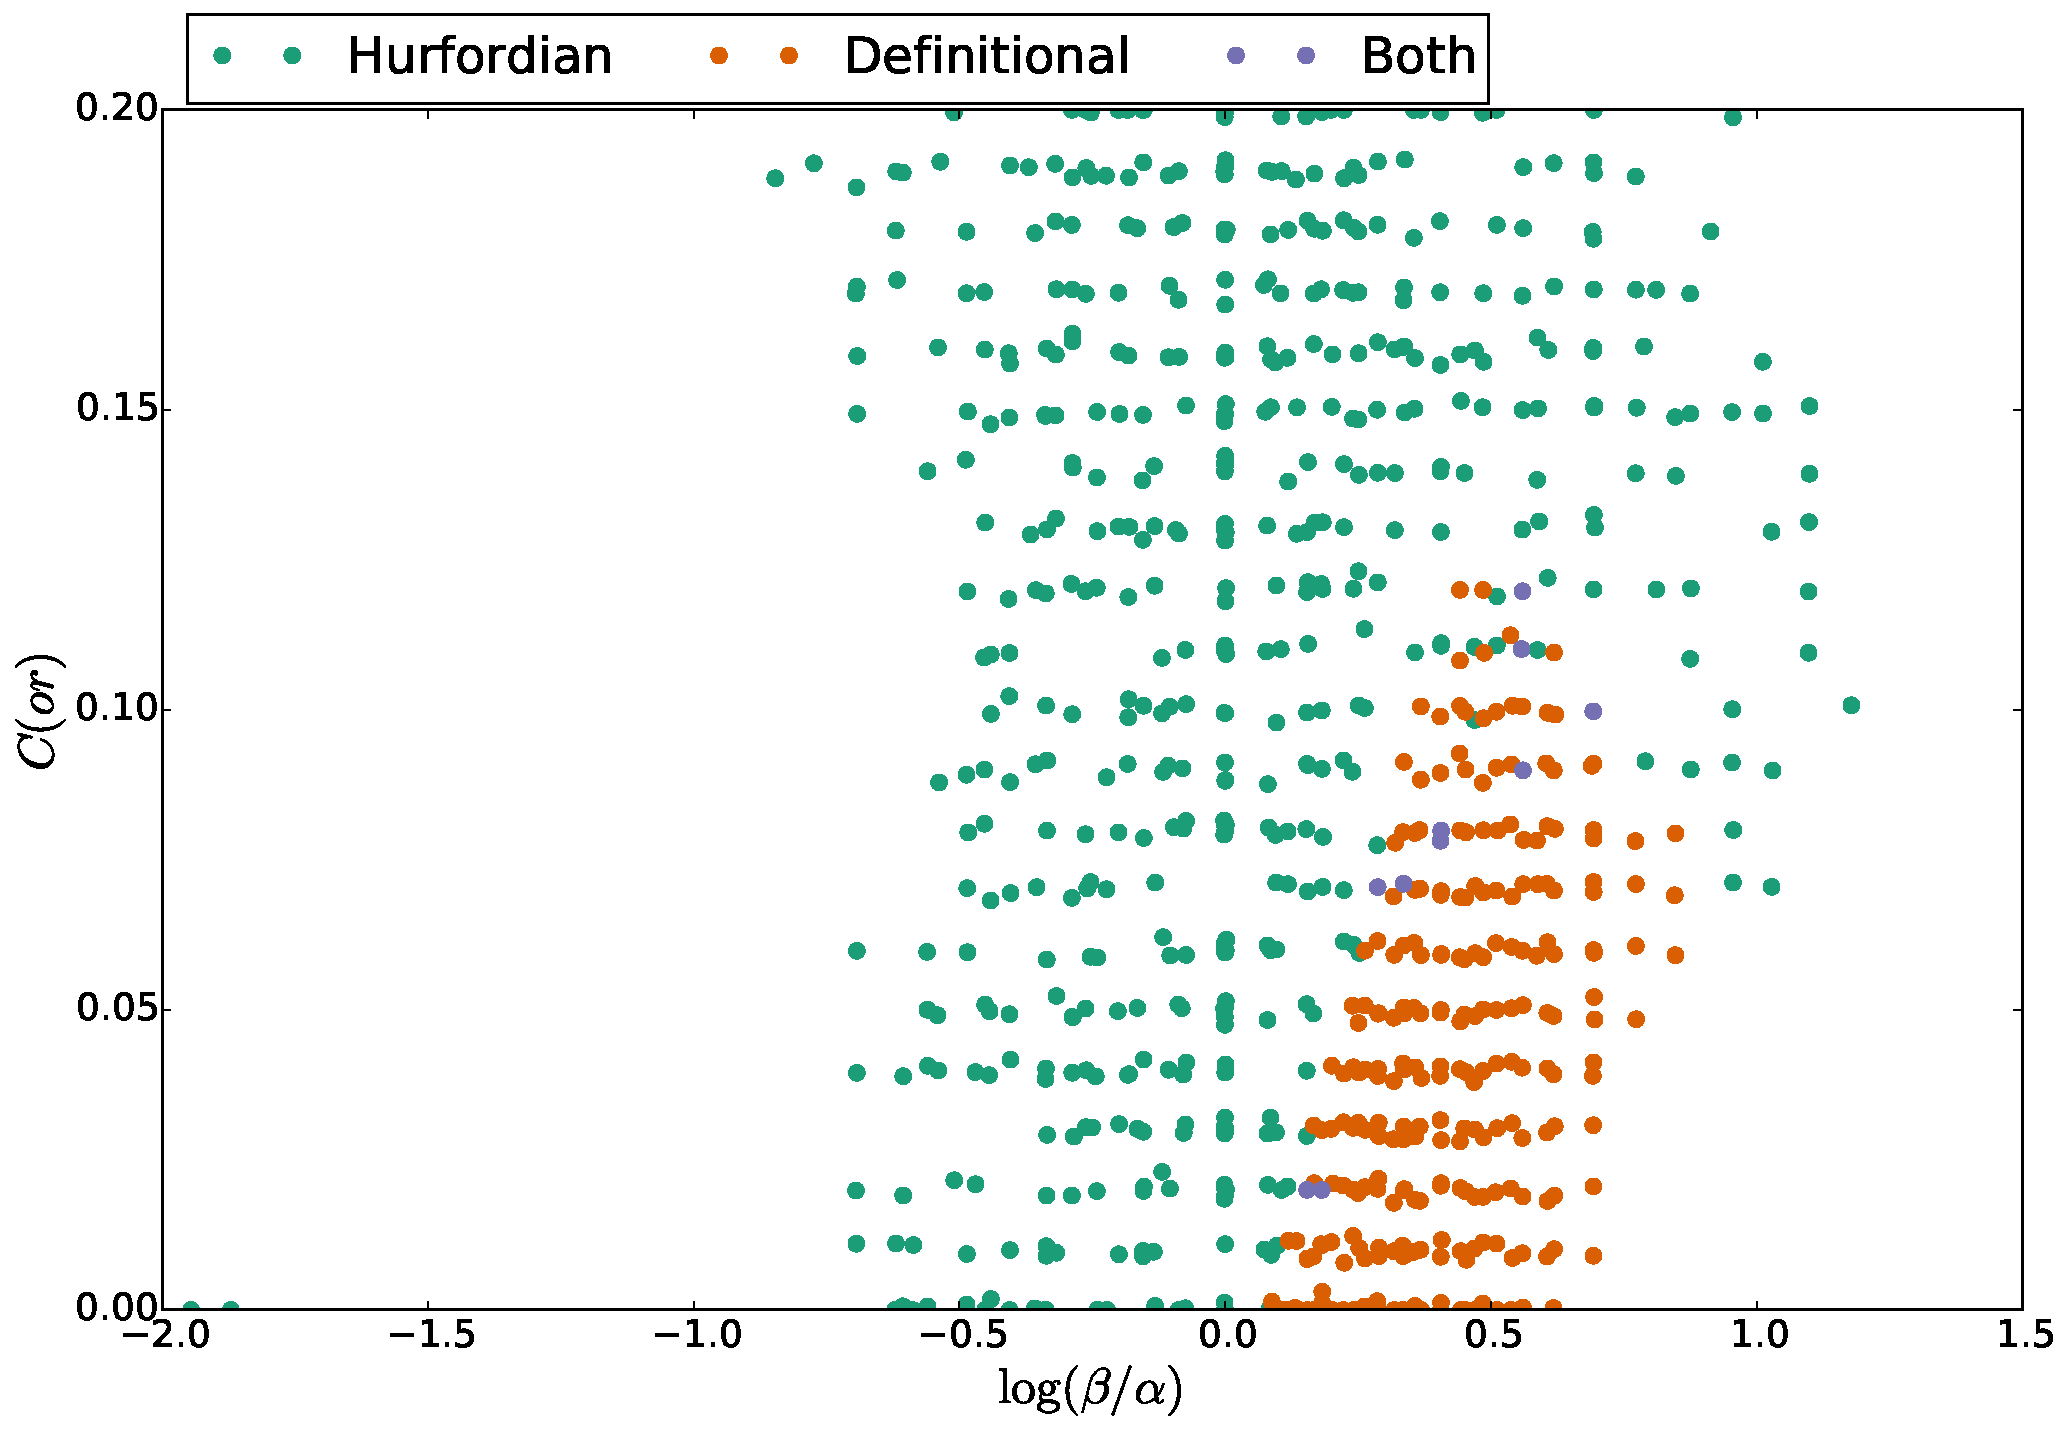
\includegraphics[width=1\textwidth]{paramexplore.pdf}

  \vspace{-4pt}

  Summarizes a search over many parameter settings using a large
  lexicon and large world space. % Definitional readings become
  % more prominent if the unknown word is constrained to have an
  % atomic meaning.

}
\end{poster}

%%%%%%%%%%%%%%%%%%%%%%%%%%%%%%%%%%%%%%%%%%%%%%%%%%%%%%%%%%%%%%%%%%%%%%
%%%%%%%%%%%%%%%%%%%%%%%%%%%%%%%%%%%%%%%%%%%%%%%%%%%%%%%%%%%%%%%%%%%%%%

\footnotesize
\setlength{\bibsep}{0pt}
\nocite{*}
\bibliographystyle{plain}
\bibliography{../levy-potts-pragdisj-bib}

\end{document}


